\documentclass[a4paper]{article}
\usepackage{graphicx}

\begin{document}

understood code

added acceptance test

unit tests

\section{Code Refactor}
included above?

\section{New Code Added}

The main aim in adding new code to the project was to enable passing of all tests.
We added glue code, which enabled us to test the features of the
system -- the test reports were now ``going red'' as the features hadn't been implemented,
rather than as a result of a lack of glue code. We were then able to focus on the
feature implementation, extending the system so that the tests passed. 

A specification for the new system features was also written. This document explains
to clients the new implementation of the system, indicating how charges would differ
from the old system. It is a high level overview of what function the change performs
and ignores lower level explanations. This would be a good introductory document
for other developers unfamiliar with the system to look at, to quickly understand
the system outputs.

\section{Anything else?}

\subsection{Circular Dependencies}

A key takeaway from the course so far has been increasing the maintainability of
code -- reducing coupling and increasing cohesion being a great area of focus on
this point. As in the last coursework, we utilised developer tool \emph{stan4j} as
well as IntelliJ's dependency analyser.

\begin{figure}[h]
\centering
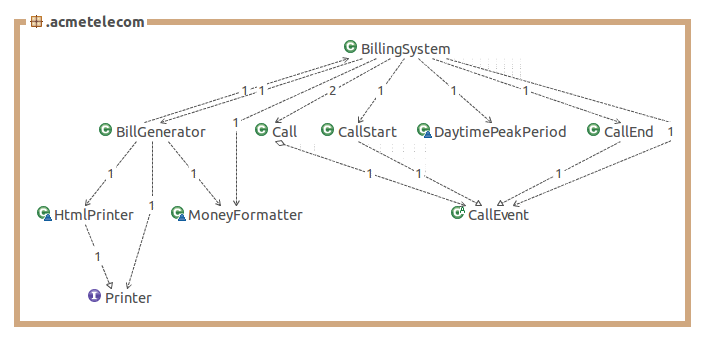
\includegraphics[width=\textwidth]{dependency_graph}
\caption{The dependency graph as indicated by stan4j}
\end{figure}

We observed a circular dependency between BillingSystem and BillingGenerator which
could potentially cause issues if we were to replace one of these classes. Our
first move was to remove this dependency by moving LineItem, which is a static inner class
of BillingSystem, into it's own class. 


\subsection{Maven}

One of the first extra features we implemented in the code base was to
convert the project to a maven project. A couple of members of our team
had prior experience with creating maven projects so the process was fairly
straightforward. 

Once the pom file had been created and the file system restructured, we were
able to import all external (publicly available) libraries from the maven repo
stored elsewhere in our filesystem. This allowed us to clear up the library folder.
Obviously, we would need a location to store our \emph{external.jar}. Assuming this
jar only needs to be used within our project, we created a local repository to
the project and pointed to it within our pom file, allowing maven to build our
project with this dependency. In a industrial environment, we would likely set
up a shared repository across the company where this jar file would be stored
and accessible by anyone, allowing us to remove it from our project.

\begin{figure}[h]
\begin{verbatim}  
<repositories>
  <repository>
    <id>in-project</id>
    <name>Custom JARs</name>
    <url>file://${project.basedir}/lib</url>
    <releases><enabled>true</enabled><updatePolicy>always</updatePolicy></releases>
    <snapshots><enabled>true</enabled><updatePolicy>always</updatePolicy></snapshots>
  </repository>
</repositories>

<dependencies>
  <dependency>
    <groupId>com.acmetelecom</groupId>
    <artifactId>external</artifactId>
    <version>1.0.0</version>
  </dependency>
...
</dependencies>
\end{verbatim}
\caption{Specifying project dependencies via the pom.xml}
\end{figure}
A feature of maven is the dependency plugin. This allows testing of our pom file
(which we initially set up to depend on all jars found in the initial lib folder)
to ensure there are no unnecessary or missing dependencies. Running the
dependency analyser enabled us to remove a number of the info.cukes jars and
the jchrnoic jar. This could have been performed manually by examining all imports
in the project, but the maven analyser hugely sped up the process.

The use of maven also enabled easy integration of our projects with eclipse. We
no longer had to manually add new dependencies to our build path etc. with each
pull, it was all taken care for us, ensuring the correct dependencies were used
and freeing up our time to tackle the main challenge.

Further to this, we were also encouraged to add testing to our code as maven would
automatically run these when building. We coupled this with Travis CI to great effect,
as discussed next.

\subsection{Travis Continuous Integration}

An issue with running maven on it's own, is that it's very easy for a developer
to forget to run the tests before pushing their code. This results in failing tests 
and bad code being pushed, which obviously isn't ideal and would only be discovered
once another user pulls and tries to build the project.

To circumvent this problem, we decided to go with \emph{Travis}, a continuous
integration tool. Travis was able to integrate well with github, which we were
using as a our centralised repo, and run tests on every pushed version. When one
of these builds failed, either through compilation errors (usually a file which
hadn't been added to the repo) or test failures, the whole team would receive
emails explaining what failed and who was the comitter who introduced the fault.
This ensured everyone took ownership of their work and massively reduced the 
number of errors pushed to the central repo.

Again, the use of Travis creates a constant reminder about testing. With emails
sent to each team member on every push, indicating test passes/failures, it is
easy to see if somebody has been going too lightly on tests. For example, if
a big change has been pushed (multiple commits, many lines added) but the number
of tests hasn't changed, it becomes clear that this is an area where more testing
is needed.

\section{Adding further features}

Further features could be added to this project after we have finished with it.
A number of approaches are/can be taken to ensure reliability and maintainability
in future.

\subsection{Implemented}

All approaches taken in completing the current project are pivotal in the management
of future code changes. In refactoring the code, we have made the structure of
the project easy to extend as needed. For example the Printer class now contains
a printBill method, generating the entire bill, as a future enhancement may be to
give the whole bill in a format other than html (e.g. PDF).

Maven and Travis CI, as explained previously, increase reliability with continuous
testing of code. Maven also aids in the maintainability of code, managing external
dependencies.

\subsection{Test Driven Development (TDD)}

One approach we didn't take however would recommend utlising in future is a pure
TDD approach. As we were focussing on increasing the maintainability and reliability
of the code, we had no issue adding tests where needed (I think?). In future however,
other developers may see this as a lower priority goal of the project and so could
easily turned the code into a big unmaintainable mess. In enforcing TDD, we could
ensure that those who otherwise wouldn't focus on this aspect, kept their code
maintainable and correct. TDD also forces developers to think about what exactly
they want their code to achieve before diving into the work -- this improves
reliability not only through tests, but also through creating strict pre and
post conditions for functions. 

\end{document}